% !TeX spellcheck = da_DK
\subsection{Offsetjustering}
\subsubsection{Teori og design} \label{Offset_Teori_Design}
Det analoge signal, der kommer fra accelerometeret, har et indbygget offset, som gør, at outputtet giver halvdelen af accelerometerets spændingsforsyning. For at kunne forstærke signalet, der både skal indeholde positive og negative værdier, er det nødvendigt at ændre dette offset. På denne måde kan  accelerometeret i steady state ved $0$g påvirkning have et outputsignal på $0$V. Måden hvorpå dette nye offset indføres er ved anvendelse af et differensforstærker kredsløb, som ses på \figref{fig:Differensforstaerker_generisk}. Dette kredsløb kan tage et af inputsignalerne, kaldet $V_{b}$ på figuren, og  fratrække det andet inputsignal, kaldet $V_{a}$ på figuren, som vil fungere som en referenceværdi.

\begin{figure}[H]
\centering
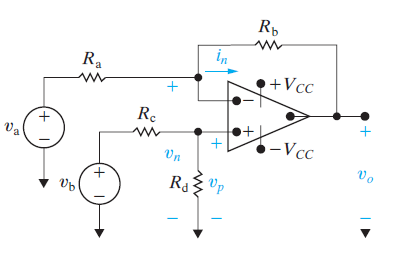
\includegraphics[scale=1.3]{figures/cProblemloesning/Differensforstaerker_generisk.png}
\caption{På figuren er et generisk differens forstærker kredsløb illustreret. \cite{Nilsson2011}}
\label{fig:Differensforstaerker_generisk}
\end{figure}

\noindent Ligning \ref{eq:Diff1} er den simplificeret ligning for differensforstærker kredsløbet, hvor $\frac{R_a}{R_b} = \frac{R_c}{R_d}$;

\begin{equation}\label{eq:Diff1}
V_o = \frac{R_b}{R_a} \cdot (v_b - v_a)
\end{equation}

\noindent Der kan heraf ses, at forstærkningen på signalet kan bestemmes ved at vælge modstandene $R_a \text{og} R_b$, og at det er spændingen $V_{a}$, der trækkes fra spændingen $V_{b}$. \\
I dette tilfælde kræves der ikke en forstærkning, hvorfor modstandene $R_{a}$ og $R_{b}$ skal være det samme. Da signalet ikke skal inverteres sendes accelerometerets output ind i den ikke-inverterende kanal. Offsettet, som i dette tilfælde er en referenceværdi på $1.6325$V jævnført \ref{Mean_tid_0g} på side \pageref{Mean_tid_0g}, sendes ind i den inverterende kanal. Dette illustreres på figur \ref{fig:Offset_generisk}:
\begin{figure}[H]
\centering
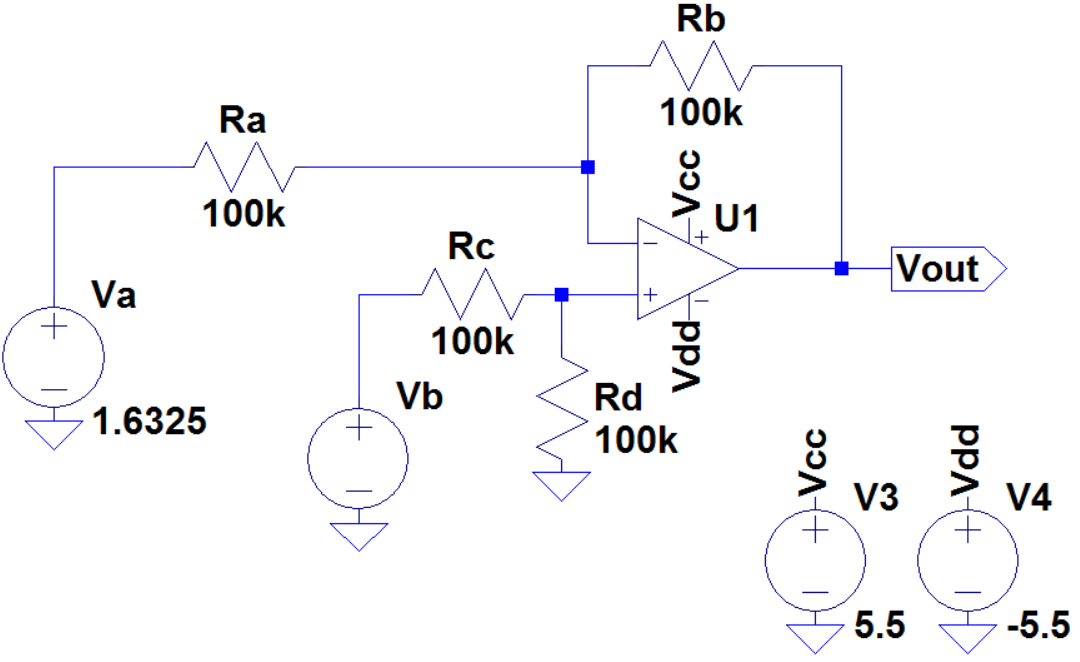
\includegraphics[scale=0.45]{figures/cProblemloesning/Offset_generisk.png}
\caption{På figuren ses offsetjusteringens opbygning. $V1$ er referenceværdien, som sættes til $1.6325$V, og $Va$ er outputtet fra accelerometeret, som vil skabe inputtet $V2$ til operationsforstærkeren. Modstandene i kredsløbet er ens, hvilket medfører, at signalet ikke forstærkes. Grunden til at spændingsforsyningen er $\pm5.5$V er, at spændingsforsyningen til hele systemet er designet til at give et output på $\pm5.5$V, hvor arbejdsområdet er $\pm3$V. Derved sikres det, at ønskede signal ikke går i mætning.}
\label{fig:Offset_generisk}
\end{figure}

\subsubsection{Simulering}
Der foretages tre simuleringer i LTspice - en for hhv. den højeste- og laveste spænding, som accelerometret kan give for øvelserne. Dette vil svare til 1g påvirkning af accelerometerets x akse - altså $90^{\circ}$ rotation. Derudover foretages der en simulering for 0g påvirkning, hvilket svarer til $0^{\circ}$ rotation. Resultaterne ses i \tableref{Tab:offset_sim}.
\begin{table}[H]
	\centering
	\begin{tabular}{|l|l|l|l|l|}
		\hline
		\multicolumn{1}{|c|}{\textit{Inputsignal}} & \multicolumn{1}{c|}{\textit{Offset}} & \multicolumn{1}{c|}{\textit{Forventet outputsignal}} & \multicolumn{1}{c|}{\textit{Outputsignalet}} & \multicolumn{1}{c|}{\textit{Afvigelse}} \\ \hline
		$1.9638$V     & $1.6325$V    & $0.3313V$V    & $0.3313$V       & $0$\%              \\ \hline
		$1.6325$V     & $1.6325$V    & $0$V          & -$22.949\mu$V   & $\approx 0$\%      \\ \hline
		$1.3092$V     & $1.6325$V    & -$0.3233V$V   & -$0.3233$V      & $0$\%                \\ \hline
	\end{tabular}
	\caption{I tabellen ses resultaterne fra simuleringerne af offsettet med forskellige inputs.}
	\label{Tab:offset_sim}
\end{table}
\noindent Der ses, at der ingen afvigelse er imellem de forventede outputsignal og det simulerede outputsignal. Dette betyder, at kredsløbet fungerer rent teoretisk med ideelle komponenter, som bliver anvendt i LTspice. På \figref{fig:Offset_simulering} ses simuleringen af $1.6325$V input fra accelerometret.
 
\begin{figure}[H]
\centering
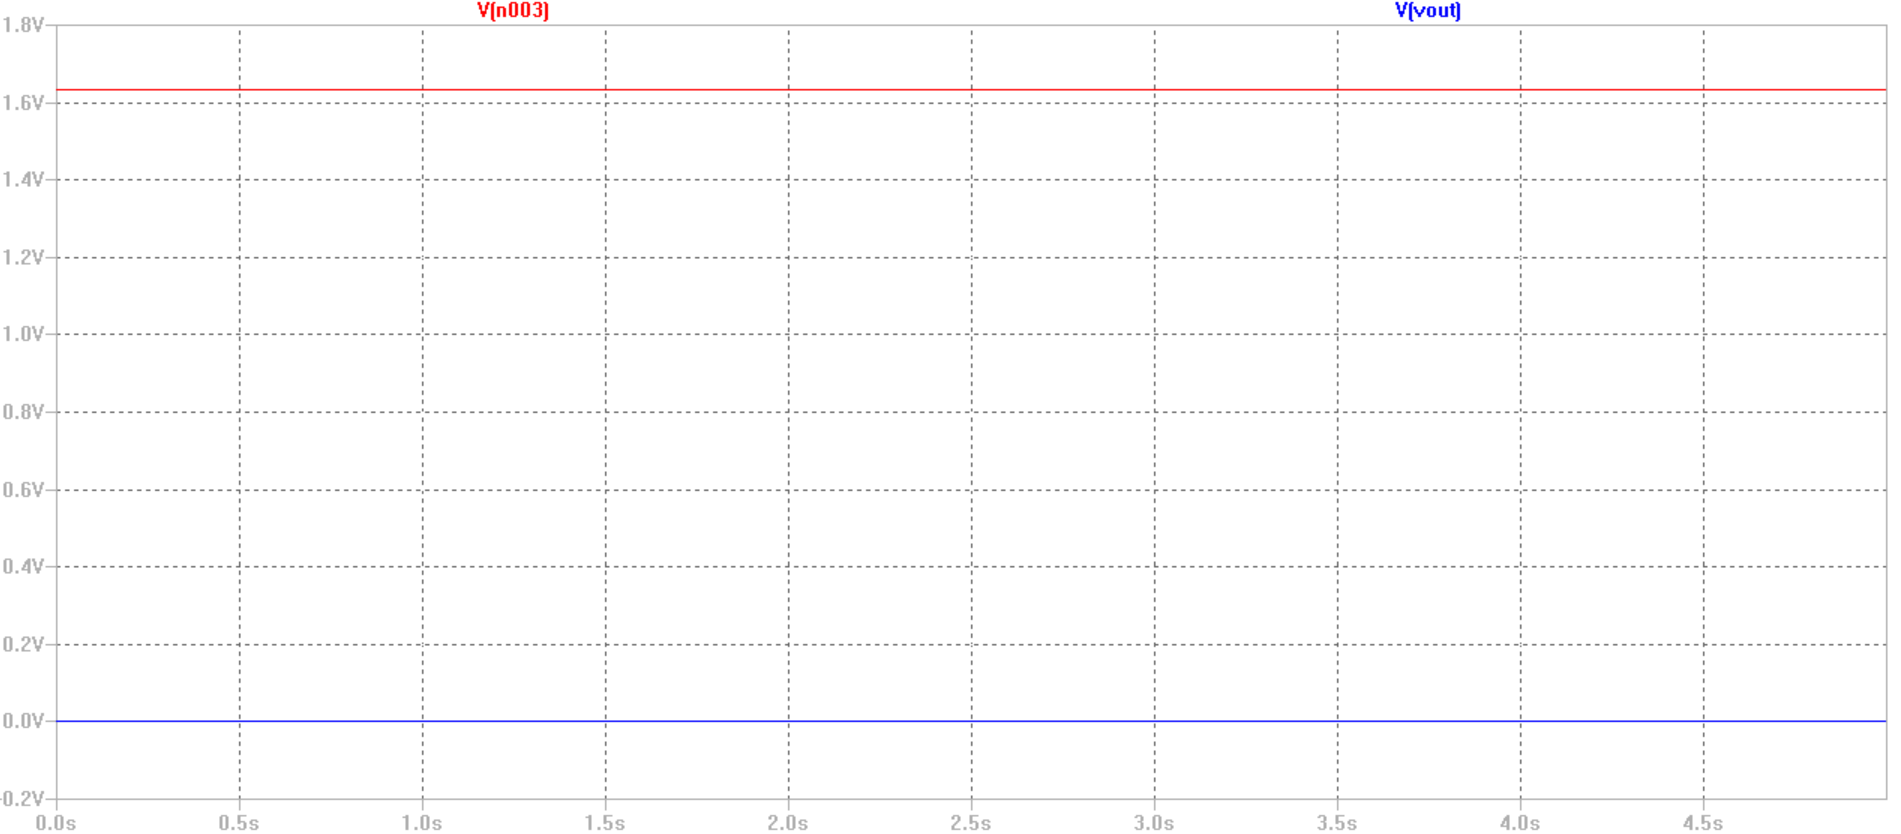
\includegraphics[scale=0.3]{figures/cProblemloesning/Offset_simulering.png}
\caption{På figuren ses en simulering af $1.6325$V input, hvilket giver et output på $\approx 0$V.}
\label{fig:Offset_simulering}
\end{figure}

\subsubsection{Implementering og test}
I implementeringen arbejdes der med reelle komponenter. Derfor vil der være afvigelser fra resultaterne imellem testen med ideelle komponenter i dette afsnit og testen med reelle komponenter i simuleringen. \\
Der ses på \figref{fig:Offset_generisk}, at der skal benyttes fire modstandere på $100$K$\Omega$ til opbygningen af offsettet. Disse blev målt inden testen, hvilket fremgår i \tableref{Tab:modstand_offset}.
\begin{table}[H]
	\centering
	\begin{tabular}{|l|l|l|}
		\hline
		\textit{Teoretisk} & \textit{Ved måling} & \textit{\% afvigelse} \\ \hline
		$100$K$\Omega$       & $99.8$K$\Omega$       & $0.2$\%               \\ \hline
		$100$K$\Omega$       & $99.7$K$\Omega$       & $0.3$\%               \\ \hline
		$100$K$\Omega$       & $99.7$K$\Omega$       & $0.3$\%               \\ \hline
		$100$K$\Omega$       & $99.7$K$\Omega$       & $0.3$\%               \\ \hline
	\end{tabular}
	\caption{I tabellen ses der, at alle fire modstandere afviger lidt fra deres teoretiske værdi, hvilket er forventet af reelle komponenter. Kravet til disse fire modstandere var dog, at de skulle være ens således at der ikke sker en forstærkning. Disse modstandere accepteres derfor.}
	\label{Tab:modstand_offset}
\end{table}
\noindent Herefter implementeres kredsløbet. Til opsamling af signalet benyttes en computer med ScopeLogger, hvorefter dataen bliver behandlet i Matlab. I testen blev der foretaget 3 målinger for de to spændingsniveauer. Herefter blev gennemsnittet for hver måling udregnet, som lægges sammen og til slut også tages gennemsnittet af. Dette giver den endelige værdi, som står under "Output" i \tableref{Tab:Offset_test}.
\begin{table}[H]
	\centering
	\begin{tabular}{l|l|l|l|l|l|}
		\cline{2-6}
		& \textit{\begin{tabular}[c]{@{}l@{}}Ønskede\\ input\end{tabular}} & \textit{Input} & \textit{\begin{tabular}[c]{@{}l@{}}Forventet\\ output\end{tabular}} & \textit{Output} & \% afvigelse \\ \hline
		\multicolumn{1}{|l|}{\textit{\begin{tabular}[c]{@{}l@{}}$V1$\\ ref\end{tabular}}}    & $1.6325$V    & $1.6352$V    & $\times$    & $\times$   & $\times$     \\ \hline
		\multicolumn{1}{|l|}{\multirow{2}{*}{\textit{\begin{tabular}[c]{@{}l@{}}$V2$\\ signal\end{tabular}}}} & $1.9638$V   & $1.9629$V    & $0.3277$V   & $0.3252X$V   & $0.76\%$     \\ \cline{2-6} 
		\multicolumn{1}{|l|}{}   & $1.6325$V   & $1.6352$V    &  $0$V        & -$0.0013V$V  & $\approx0\%$     \\ \cline{2-6} 
		\multicolumn{1}{|l|}{}   & $1.3092$V   &$1.3097X$V    & -$0.3255$V   & -$0.3263X$V     & $0.25\%$     \\ \hline
	\end{tabular}
	\caption{I tabellen ses en oversigt over det udregnede resultat for de to spændingsniveauer.}
	\label{Tab:Offset_test}
\end{table}
\noindent I \tableref{Tab:Offset_test}\fxnote{NTK: Det forventede output er regnet således, at den inpu det er udregnet udfra hvad i reelt har af input og reference, derefter tjekker vi om det vi målte passer med det vi fik ud} betegner "$V1$ / ref." referencespændingen, som sendes ind i den inverterende kanal. "$V2$ / signal." betegner det mindste og største output, som accelerometret kan give ved $\pm90^{\circ}$. Derudover indsendes en spænding, som svarer til reference spændingen. Disse tre spændinger bliver sendt ind i den ikke-inverterende kanal. Det "Ønskede input" er beregnet i afsnit \ref{Sec_Pilot_Data} på side \pageref{Sec_Pilot_Data} og burde være det, som sendes ind i $V2$. "Input" er den spænding, som sendes ind fra spændingsforsyningen, og "Forventet output" udregnes ved at trække inputtet fra reference spændingen fra inputtet fra det indsendte signal. "Output" er slutresultatet efter gennemsnitsberegninger og "afvigelsen" kan derved beregnes. \\
Der ses i \tableref{Tab:Offset_test}, at der er en meget lav afvigelse imellem outputtet og det forventede output for hver inputspænding. Disse afvigelser ligger inde for tolerancen for offsettet beskrevet i afsnit \ref{OpsamlingsAfs} på side \pageref{OpsamlingsAfs}. Derfor anses disse afvigelser som acceptable.